%% MorsEye paper (PRD §8). ACM acmart, sigconf, 4-6 pages + references. Build: latexmk (see latexmkrc).
%%
%% RULES (PRD §2, §8.5)
%%  - Since 24 Oct 2026 (PRD §2) the AI agent may draft any section; Saksham reviews and edits it. Every
%%    section below was drafted by the agent on 25 Oct 2026 (listed in AI_USE.md and in the AI-use section).
%%  - Figures (figures/C*, F1) and tables (tables/case_*) are generated by `python -m analysis.case_study`
%%    (after `python -m analysis.public_blinks`). Do not edit them.
%%  - Every number in the text comes from analysis/out/results.json via \CS{key} (tables/case_numbers.tex).
%%  - No "state of the art" claims and no claims about users with disabilities.
%%  - [HUMAN] marks what only Saksham can do: read every cited paper and replace its placeholder BibTeX,
%%    finalise title, affiliation, CCS concepts and keywords, and review every section.

\documentclass[sigconf,nonacm]{acmart}

\graphicspath{{figures/}}
\renewcommand{\topfraction}{0.9}
\renewcommand{\dbltopfraction}{0.9}
\renewcommand{\textfraction}{0.1}
\renewcommand{\floatpagefraction}{0.8}
\renewcommand{\dblfloatpagefraction}{0.8}
% Generated by analysis/case_outputs.py from analysis/out/results.json. Do not edit.
\makeatletter
\newcommand{\CS}[1]{\@ifundefined{CS@#1}{\textbf{??#1??}}{\csname CS@#1\endcsname}}
\expandafter\def\csname CS@rejectMs\endcsname{200}
\expandafter\def\csname CS@dotMaxMs\endcsname{600}
\expandafter\def\csname CS@dashMaxMs\endcsname{1400}
\expandafter\def\csname CS@cmdMs\endcsname{2000}
\expandafter\def\csname CS@pubVideos\endcsname{8}
\expandafter\def\csname CS@pubPeople\endcsname{4}
\expandafter\def\csname CS@pubMinutes\endcsname{40}
\expandafter\def\csname CS@pubBlinks\endcsname{408}
\expandafter\def\csname CS@pubFps\endcsname{31}
\expandafter\def\csname CS@pubBlink-p5\endcsname{192}
\expandafter\def\csname CS@pubBlink-median\endcsname{272}
\expandafter\def\csname CS@pubBlink-p95\endcsname{560}
\expandafter\def\csname CS@pubBelowReject\endcsname{9\%}
\expandafter\def\csname CS@pub-D1-before\endcsname{11.8 [9.2, 14.2]}
\expandafter\def\csname CS@pub-D1-after\endcsname{10.2 [7.5, 12.9]}
\expandafter\def\csname CS@pub-D1-before-mean\endcsname{11.8}
\expandafter\def\csname CS@pub-D1-after-mean\endcsname{10.2}
\expandafter\def\csname CS@pub-D1-ratio\endcsname{0.86}
\expandafter\def\csname CS@pub-D1-p\endcsname{0.008}
\expandafter\def\csname CS@pub-D1-recall\endcsname{80\%}
\expandafter\def\csname CS@pub-D1-closedMedian\endcsname{272}
\expandafter\def\csname CS@pub-D1-belowReject\endcsname{16\%}
\expandafter\def\csname CS@pub-D1-meets\endcsname{no}
\expandafter\def\csname CS@pub-D3-before\endcsname{10.5 [7.5, 13.2]}
\expandafter\def\csname CS@pub-D3-after\endcsname{4.1 [2.7, 5.7]}
\expandafter\def\csname CS@pub-D3-before-mean\endcsname{10.5}
\expandafter\def\csname CS@pub-D3-after-mean\endcsname{4.1}
\expandafter\def\csname CS@pub-D3-ratio\endcsname{0.39}
\expandafter\def\csname CS@pub-D3-p\endcsname{0.008}
\expandafter\def\csname CS@pub-D3-recall\endcsname{87\%}
\expandafter\def\csname CS@pub-D3-closedMedian\endcsname{192}
\expandafter\def\csname CS@pub-D3-belowReject\endcsname{60\%}
\expandafter\def\csname CS@pub-D3-meets\endcsname{yes}
\expandafter\def\csname CS@sFps\endcsname{15.0}
\expandafter\def\csname CS@sFps-calibration\endcsname{16.4}
\expandafter\def\csname CS@sFps-spontaneous\endcsname{15.1}
\expandafter\def\csname CS@sFps-deliberate\endcsname{16.4}
\expandafter\def\csname CS@sFps-mixed\endcsname{10.3}
\expandafter\def\csname CS@sFace\endcsname{99.7\%}
\expandafter\def\csname CS@sMissing\endcsname{0.06\%}
\expandafter\def\csname CS@sMinutes\endcsname{9.6}
\expandafter\def\csname CS@sCues\endcsname{84}
\expandafter\def\csname CS@sMatch\endcsname{80}
\expandafter\def\csname CS@sCalib\endcsname{20}
\expandafter\def\csname CS@s-D1-reading-before\endcsname{12.7}
\expandafter\def\csname CS@s-D1-reading-after\endcsname{2.7}
\expandafter\def\csname CS@s-D1-reading-n\endcsname{38}
\expandafter\def\csname CS@s-D1-reading-rejected\endcsname{30}
\expandafter\def\csname CS@s-D2-reading-before\endcsname{10.7}
\expandafter\def\csname CS@s-D2-reading-after\endcsname{1.0}
\expandafter\def\csname CS@s-D2-reading-n\endcsname{32}
\expandafter\def\csname CS@s-D2-reading-rejected\endcsname{29}
\expandafter\def\csname CS@s-D3-reading-before\endcsname{10.0}
\expandafter\def\csname CS@s-D3-reading-after\endcsname{0.3}
\expandafter\def\csname CS@s-D3-reading-n\endcsname{30}
\expandafter\def\csname CS@s-D3-reading-rejected\endcsname{29}
\expandafter\def\csname CS@s-D4-reading-before\endcsname{11.7}
\expandafter\def\csname CS@s-D4-reading-after\endcsname{2.0}
\expandafter\def\csname CS@s-D4-reading-n\endcsname{35}
\expandafter\def\csname CS@s-D4-reading-rejected\endcsname{29}
\expandafter\def\csname CS@s-D5-reading-before\endcsname{0.3}
\expandafter\def\csname CS@s-D5-reading-after\endcsname{0.3}
\expandafter\def\csname CS@s-D5-reading-n\endcsname{1}
\expandafter\def\csname CS@s-D5-reading-rejected\endcsname{0}
\expandafter\def\csname CS@s-D1-correct\endcsname{13/33}
\expandafter\def\csname CS@s-D1-short-none\endcsname{1}
\expandafter\def\csname CS@s-D1-short-reject\endcsname{0}
\expandafter\def\csname CS@s-D1-short-dot\endcsname{1}
\expandafter\def\csname CS@s-D1-short-dash\endcsname{13}
\expandafter\def\csname CS@s-D1-short-hold\endcsname{1}
\expandafter\def\csname CS@s-D1-short-backspace\endcsname{1}
\expandafter\def\csname CS@s-D1-long-none\endcsname{2}
\expandafter\def\csname CS@s-D1-long-reject\endcsname{0}
\expandafter\def\csname CS@s-D1-long-dot\endcsname{0}
\expandafter\def\csname CS@s-D1-long-dash\endcsname{12}
\expandafter\def\csname CS@s-D1-long-hold\endcsname{0}
\expandafter\def\csname CS@s-D1-long-backspace\endcsname{2}
\expandafter\def\csname CS@s-D2-correct\endcsname{15/33}
\expandafter\def\csname CS@s-D2-short-none\endcsname{1}
\expandafter\def\csname CS@s-D2-short-reject\endcsname{0}
\expandafter\def\csname CS@s-D2-short-dot\endcsname{3}
\expandafter\def\csname CS@s-D2-short-dash\endcsname{13}
\expandafter\def\csname CS@s-D2-short-hold\endcsname{0}
\expandafter\def\csname CS@s-D2-short-backspace\endcsname{0}
\expandafter\def\csname CS@s-D2-long-none\endcsname{2}
\expandafter\def\csname CS@s-D2-long-reject\endcsname{0}
\expandafter\def\csname CS@s-D2-long-dot\endcsname{1}
\expandafter\def\csname CS@s-D2-long-dash\endcsname{12}
\expandafter\def\csname CS@s-D2-long-hold\endcsname{0}
\expandafter\def\csname CS@s-D2-long-backspace\endcsname{1}
\expandafter\def\csname CS@s-D3-correct\endcsname{18/33}
\expandafter\def\csname CS@s-D3-short-none\endcsname{1}
\expandafter\def\csname CS@s-D3-short-reject\endcsname{0}
\expandafter\def\csname CS@s-D3-short-dot\endcsname{4}
\expandafter\def\csname CS@s-D3-short-dash\endcsname{12}
\expandafter\def\csname CS@s-D3-short-hold\endcsname{0}
\expandafter\def\csname CS@s-D3-short-backspace\endcsname{0}
\expandafter\def\csname CS@s-D3-long-none\endcsname{0}
\expandafter\def\csname CS@s-D3-long-reject\endcsname{0}
\expandafter\def\csname CS@s-D3-long-dot\endcsname{1}
\expandafter\def\csname CS@s-D3-long-dash\endcsname{14}
\expandafter\def\csname CS@s-D3-long-hold\endcsname{0}
\expandafter\def\csname CS@s-D3-long-backspace\endcsname{1}
\expandafter\def\csname CS@s-D4-correct\endcsname{17/33}
\expandafter\def\csname CS@s-D4-short-none\endcsname{1}
\expandafter\def\csname CS@s-D4-short-reject\endcsname{0}
\expandafter\def\csname CS@s-D4-short-dot\endcsname{2}
\expandafter\def\csname CS@s-D4-short-dash\endcsname{13}
\expandafter\def\csname CS@s-D4-short-hold\endcsname{1}
\expandafter\def\csname CS@s-D4-short-backspace\endcsname{0}
\expandafter\def\csname CS@s-D4-long-none\endcsname{0}
\expandafter\def\csname CS@s-D4-long-reject\endcsname{0}
\expandafter\def\csname CS@s-D4-long-dot\endcsname{0}
\expandafter\def\csname CS@s-D4-long-dash\endcsname{15}
\expandafter\def\csname CS@s-D4-long-hold\endcsname{0}
\expandafter\def\csname CS@s-D4-long-backspace\endcsname{1}
\expandafter\def\csname CS@s-D5-correct\endcsname{0/31}
\expandafter\def\csname CS@s-D1-short-p5\endcsname{602}
\expandafter\def\csname CS@s-D1-short-median\endcsname{702}
\expandafter\def\csname CS@s-D1-short-p95\endcsname{1921}
\expandafter\def\csname CS@s-D1-long-p5\endcsname{839}
\expandafter\def\csname CS@s-D1-long-median\endcsname{1242}
\expandafter\def\csname CS@s-D1-long-p95\endcsname{5572}
\expandafter\def\csname CS@s-D2-short-p5\endcsname{567}
\expandafter\def\csname CS@s-D2-short-median\endcsname{635}
\expandafter\def\csname CS@s-D2-short-p95\endcsname{1105}
\expandafter\def\csname CS@s-D2-long-p5\endcsname{726}
\expandafter\def\csname CS@s-D2-long-median\endcsname{1153}
\expandafter\def\csname CS@s-D2-long-p95\endcsname{1783}
\expandafter\def\csname CS@s-D3-short-p5\endcsname{494}
\expandafter\def\csname CS@s-D3-short-median\endcsname{664}
\expandafter\def\csname CS@s-D3-short-p95\endcsname{912}
\expandafter\def\csname CS@s-D3-long-p5\endcsname{699}
\expandafter\def\csname CS@s-D3-long-median\endcsname{1118}
\expandafter\def\csname CS@s-D3-long-p95\endcsname{2102}
\expandafter\def\csname CS@s-D4-short-p5\endcsname{544}
\expandafter\def\csname CS@s-D4-short-median\endcsname{684}
\expandafter\def\csname CS@s-D4-short-p95\endcsname{1098}
\expandafter\def\csname CS@s-D4-long-p5\endcsname{774}
\expandafter\def\csname CS@s-D4-long-median\endcsname{1126}
\expandafter\def\csname CS@s-D4-long-p95\endcsname{2731}
\makeatother

% [HUMAN] Set to false once you have reviewed and edited the draft (removes the notice under the title).
\newif\ifunreviewed
\unreviewedtrue

\settopmatter{printacmref=false}

% [HUMAN] Working title (drafted by the agent). Finalise it yourself.
\title{Deliberate or spontaneous? A duration reject window for webcam blink typing, checked on public blink videos and one recorded session}

\author{Saksham Sharma}
\affiliation{%
  \institution{BITS Pilani}
  \country{India}}
% [HUMAN] Check the affiliation; add your campus \city{...} and, if you want, an \email{...}.

\begin{abstract}
Blink-based text entry uses the eyelid as a key, but the eyelid also closes on its own many times a minute.
MorsEye is an open-source browser system that types Morse code from eye closures on a laptop webcam: it
measures closures from MediaPipe face landmarks and blendshape scores, ignores closures shorter than a reject
window, and maps longer ones to dots and dashes. A preregistered single-person study was planned, but data
collection stopped after one session without labelled closure times, so its confirmatory tests were not run. We
report what remains. On \CS{pubBlinks} annotated natural blinks of \CS{pubPeople} people in a public video
dataset (Eyeblink8; secondary, not blind), a \CS{rejectMs}\,ms reject window cut false triggers from
\CS{pub-D3-before} to \CS{pub-D3-after} per minute with a blendshape detector, but only from \CS{pub-D1-before}
to \CS{pub-D1-after} with the eye aspect ratio. In the one recorded session (exploratory), the author's cued short
closures mostly lasted longer than the \CS{dotMaxMs}\,ms dot limit, and winks closed both eyes as far as the
camera could tell.
\end{abstract}

% [HUMAN] CCS concepts and keywords: choose them yourself from the ACM CCS tool.

\begin{document}
\maketitle

\ifunreviewed
\noindent\fcolorbox{red}{white}{\parbox{\dimexpr\linewidth-2\fboxsep-2\fboxrule}{\color{red}\small
\textbf{Draft.} Every section of this text was drafted by an AI agent (Claude Code) and has not yet been
reviewed by the author. Every number is generated from the logged data by the analysis scripts.}}
\fi

%% ---------------------------------------------------------------------------------------------
\section{Introduction}

People who cannot speak or use their hands may still control their eyelids, which makes blinks a candidate
input for text entry~\cite{grauman2003,majaranta2002}. The difficulty is that the ``key'' also moves on its own:
spontaneous blinks happen many times a minute, and a system that types a symbol for each of them is unusable.
Webcam blink typing therefore has to tell deliberate closures from spontaneous ones, using only what an ordinary
laptop camera at about 30 frames per second can see.

MorsEye takes a simple approach: deliberate closures are made longer than natural blinks, and closures shorter
than a \emph{reject window} are ignored. Short and long deliberate closures become Morse dots and dashes. This
paper reports three things:
\begin{itemize}
  \item an open-source browser system that runs entirely on the device, with per-user calibration, a duration
        segmenter and a study and labelling mode (Section~\ref{sec:system});
  \item a check of the reject window on other people's natural blinks in a public video dataset
        (Section~\ref{sec:public});
  \item an exploratory account of one recorded session of the author, which shows where the default timing
        bands did not fit (Section~\ref{sec:session}).
\end{itemize}
The paper also reports, with the dated deviations, why the preregistered study it was designed around was not
completed (Section~\ref{sec:plan}).

%% ---------------------------------------------------------------------------------------------
\section{Related Work}
% [HUMAN] Drafted by the agent from general knowledge of these works. Read each paper before keeping its
% citation, check every sentence against it, replace the placeholder BibTeX, and add the recent (2020-2026)
% webcam blink-typing systems you find, saying how this work differs from each.

Soukupov\'{a} and \v{C}ech~\cite{soukupova2016} proposed the eye aspect ratio (EAR), computed from six landmarks
around each eye, as a per-frame measure of eye opening for real-time blink detection. Grauman et
al.~\cite{grauman2003} used blinks and eyebrow raises from video as an interface for people with severe motor
impairments, and Majaranta and R\"{a}ih\"{a}~\cite{majaranta2002} reviewed design issues in eye typing. Annotated
blink videos, such as Eyeblink8~\cite{drutarovsky2014} and the larger Researcher's Night set~\cite{fogelton2016},
were built to evaluate blink detectors; they contain natural blinks only, not deliberate ones, which is how they
are used here.

%% ---------------------------------------------------------------------------------------------
\section{System}\label{sec:system}

\begin{figure*}[t]
  \centering
  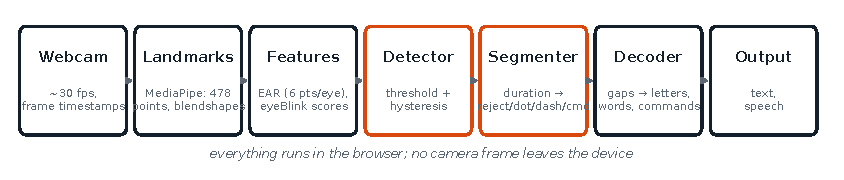
\includegraphics[width=\textwidth]{F1_pipeline}
  \Description{Block diagram: webcam, landmarks, features, detector, segmenter, decoder, output, all in the browser.}
  \caption{The MorsEye pipeline. Everything runs in the browser; no camera frame leaves the device.}
  \label{fig:pipeline}
\end{figure*}

MorsEye runs in the browser (Fig.~\ref{fig:pipeline}). Each camera frame is timestamped and passed to
MediaPipe's face landmarker~\cite{mediapipe}, which returns face landmarks and blendshape scores on the device.
Two signals are computed per frame: the mean EAR of both eyes~\cite{soukupova2016}, and the larger of the two
\texttt{eyeBlink} blendshape scores.

\paragraph{Detectors.} A detector marks the eyes closed when its signal crosses a threshold, with hysteresis so
that noise near the threshold does not split one closure into several. Closure durations come from frame
timestamps, not frame counts. Five detectors are compared: D1, EAR with the fixed threshold 0.21; D2, EAR with a
calibrated threshold; D3, blendshape with the fixed threshold 0.5; D4, blendshape with a calibrated threshold; and
D5, a wink detector that accepts a closure of one eye only while the other eye's score stays below 0.3.

\paragraph{Calibration.} The user makes ten cued short and ten cued long closures and then keeps the eyes open
for 15\,s. The threshold is placed halfway between the median open value and the median of the closures' peak
values, with hysteresis of 10\% of that range.

\paragraph{Segmenter and decoder.} Each closure is classified by duration. With the default bands, closures under
\CS{rejectMs}\,ms are ignored (the reject window), under \CS{dotMaxMs}\,ms are dots, under \CS{dashMaxMs}\,ms are
dashes, under \CS{cmdMs}\,ms are a ``hold'' (two holds in a row pause input), and longer ones delete the last
character. A pause
after a symbol ends the letter, and a longer pause adds a space.

\paragraph{Study and labelling modes.} A study mode runs the protocol with full-screen cues and logs every
frame's features (never the image) with cue and block times. A local video can be recorded for labelling, but it
stays on the laptop and is never published. A labelling tool shows the video next to the signal traces for marking
closure onsets, offsets and types by hand.

%% ---------------------------------------------------------------------------------------------
\section{The Planned Study and What Happened}\label{sec:plan}

The evaluation was preregistered on 24 Oct 2026, before the first session (\texttt{docs/preregistration.md}).
Because no volunteers were available, it was designed as a case study of one person, the author:
\begin{itemize}
  \item 6--8 detection sessions, each with a calibration block, a reading block with no cues, a block of 40 cued
        short, long, left-wink and right-wink closures, and a reading block with occasional cues;
  \item five days of typing practice;
  \item a check on public blink videos.
\end{itemize}
Confirmatory hypotheses compared calibrated with fixed thresholds (H1), blendshape with EAR (H2), and detection
with and without the reject window (H3).

Data collection stopped after the first detection session, at the author's decision. In that session the author
checked the response type to each cue in the labelling tool, but did not mark closure onsets and offsets.
Consequently:
\begin{itemize}
  \item no session has labelled closure times, so H1, H2 and H3 on the author's data were \emph{not tested}, and
        the minimum of six sessions was not met;
  \item the typing study was not run.
\end{itemize}
These changes, and smaller ones (no pilot session; a corrected count of missing frames), are recorded with dates
in the preregistration's Deviations section. What remains is the public-video analysis, which the
preregistration lists as secondary and not blind, and the single session, which is reported as exploratory.

%% ---------------------------------------------------------------------------------------------
\section{Natural Blinks in Public Videos}\label{sec:public}

\paragraph{Data and method.} Eyeblink8~\cite{drutarovsky2014} contains \CS{pubVideos} videos of \CS{pubPeople}
people (one wearing glasses) at home, \CS{pubMinutes} minutes in total at about \CS{pubFps}\,fps, with
\CS{pubBlinks} annotated natural blinks. The app's features were extracted from every frame with the same
MediaPipe version and model as the browser, and the two fixed-threshold detectors (D1, D3) and the segmenter were
run on them. Calibrated detectors could not be run, because the videos contain no deliberate closures to
calibrate from. Every blink in the videos is spontaneous, so every detected closure that the segmenter does not
reject is a false trigger. False triggers per minute are computed per video, with and without the reject window,
and summarised as the mean over videos with a 95\% percentile bootstrap CI (10,000 resamples).

This analysis is secondary and \emph{not blind}: before the preregistration was written, the AI agent that built
the analysis had already computed the annotated blink durations and run both detectors on one of the videos. The
blind version of this check, on the Researcher's Night dataset~\cite{fogelton2016}, has not been done.

\paragraph{Results.} The annotated blinks lasted a median of \CS{pubBlink-median}\,ms (5th--95th percentile
\CS{pubBlink-p5}--\CS{pubBlink-p95}\,ms); \CS{pubBelowReject} were shorter than \CS{rejectMs}\,ms.
Table~\ref{tab:public} and Fig.~\ref{fig:public} give false triggers per minute. With the blendshape detector
(D3), the reject window lowered them from \CS{pub-D3-before} to \CS{pub-D3-after} per minute (ratio of means
\CS{pub-D3-ratio}). With the EAR detector (D1), they fell only from \CS{pub-D1-before} to \CS{pub-D1-after} (ratio
\CS{pub-D1-ratio}). For both detectors the rate fell in all eight videos (Wilcoxon signed-rank $p = \CS{pub-D1-p}$
for D1 and $\CS{pub-D3-p}$ for D3, the smallest possible with eight videos), but only D3 met the preregistered criterion of at least halving the rate. The
four people are not a sample of a population, and the eight videos are not independent, so these intervals
describe these recordings only.

The difference between the detectors comes from how long each one measures a blink to be. D3 measured the
detected blinks as a median of \CS{pub-D3-closedMedian}\,ms, and \CS{pub-D3-belowReject} fell under the reject
window. D1 measured them as \CS{pub-D1-closedMedian}\,ms, and only \CS{pub-D1-belowReject} fell under it. The fixed
EAR threshold registers the eye as closed for longer, so a reject window tuned for one signal does not transfer to
the other.

\begin{figure}[t]
  \centering
  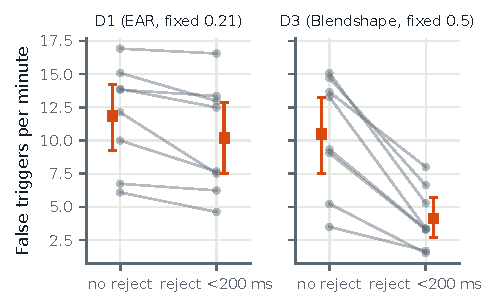
\includegraphics[width=\columnwidth]{C1_public_false_triggers}
  \Description{Two panels of paired dots, one line per video, showing false triggers per minute without and with the 200 ms reject window, for D1 (EAR, fixed 0.21) and D3 (blendshape, fixed 0.5), with the mean and 95 percent CI. All lines go down; the D3 lines go down much more.}
  \caption{Eyeblink8: false triggers per minute on natural blinks, without and with the reject window. Grey lines
  are videos; squares are means with 95\% bootstrap CIs over videos.}
  \label{fig:public}
\end{figure}

\begin{table}[t]
  \caption{Eyeblink8 videos and false triggers per minute (without $\to$ with the reject window).}
  \label{tab:public}
  \small
  \resizebox{\columnwidth}{!}{\begin{tabular}{lllrrll}
\toprule
Video & Glasses & Min & fps & Blinks & D1 FT/min & D3 FT/min \\
\midrule
1 & no & 8.9 & 31.2 & 38 & 6.1 $\to$ 4.6 & 3.5 $\to$ 1.7 \\
2 & no & 6.4 & 31.2 & 88 & 13.8 $\to$ 13.3 & 13.7 $\to$ 8.0 \\
3 & no & 5.2 & 31.2 & 65 & 12.1 $\to$ 7.5 & 9.0 $\to$ 3.3 \\
4 & no & 3.0 & 31.2 & 31 & 10.0 $\to$ 7.7 & 9.3 $\to$ 3.3 \\
8 & no & 5.9 & 31.2 & 30 & 6.7 $\to$ 6.2 & 5.2 $\to$ 1.5 \\
9 & no & 2.9 & 31.2 & 41 & 15.1 $\to$ 13.0 & 15.1 $\to$ 5.3 \\
10 & no & 5.0 & 31.2 & 72 & 13.9 $\to$ 12.5 & 13.3 $\to$ 3.4 \\
11 & yes & 2.7 & 31.2 & 43 & 16.9 $\to$ 16.6 & 14.7 $\to$ 6.6 \\
\midrule
\multicolumn{5}{l}{Mean [95\% CI] over videos} & 11.8 [9.2, 14.2] $\to$ 10.2 [7.5, 12.9] & 10.5 [7.5, 13.2] $\to$ 4.1 [2.7, 5.7] \\
\bottomrule
\end{tabular}
}
\end{table}

%% ---------------------------------------------------------------------------------------------
\section{One Recorded Session (Exploratory)}\label{sec:session}

\paragraph{Session.} The author (able-bodied, no glasses) recorded one detection session of \CS{sMinutes}
minutes with a \CS{sCamera} laptop camera at about \CS{sDistance}\,cm, in front lighting. A face was found in
\CS{sFace} of frames. The camera did not deliver 30\,fps: it ran at \CS{sFps-calibration}\,fps in the calibration
block, and fell to about 10\,fps in the last minute of the first reading block and the whole of the second
(median per block: reading \CS{sFps-spontaneous}, cued \CS{sFps-deliberate}, mixed \CS{sFps-mixed}\,fps;
Fig.~\ref{fig:fps}). The video file shows the same pattern, so the drop came from the camera's exposure, not from
the app.

Everything in this section comes from one session of one person, without confidence intervals, and is
exploratory. Closure durations here are \emph{measured by the detectors}, not labelled, so they inherit each
detector's measurement error (Section~\ref{sec:public}).

\begin{figure}[t]
  \centering
  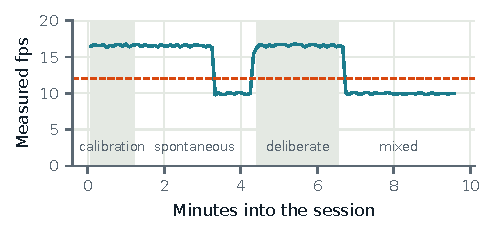
\includegraphics[width=\columnwidth]{C3_session_fps}
  \Description{Line plot of measured frame rate over the 10-minute session, with the four blocks shaded. The rate is about 16.5 fps, drops to about 10 fps near the end of the first reading block, recovers in the cued block and stays at 10 fps through the mixed block. A dashed line marks 12 fps.}
  \caption{Session 1: measured frame rate by block. The dashed line is the preregistered 12\,fps exclusion
  limit for a session's median.}
  \label{fig:fps}
\end{figure}

\paragraph{Responses to cues.} The author checked the response to every cue in the labelling tool
(Table~\ref{tab:responses}): \CS{sMatch} of \CS{sCues} responses were of the cued type.

\begin{table}[t]
  \caption{Session 1: cued type against the response type checked by the author (counts).}
  \label{tab:responses}
  \small
  \begin{tabular}{lrrrrr}
\toprule
Cue & \multicolumn{5}{c}{Response checked by the author} \\
 & short & long & wink-L & wink-R & none \\
\midrule
short & 24 & 1 & 0 & 0 & 1 \\
long & 0 & 26 & 0 & 0 & 0 \\
wink-L & 1 & 0 & 15 & 0 & 0 \\
wink-R & 0 & 0 & 1 & 15 & 0 \\
\bottomrule
\end{tabular}

\end{table}

\paragraph{Reading without cues.} The first reading block had no cues, so every closure detected in it counts as
spontaneous. The both-eye detectors found \CS{s-D3-reading-n} (D3) to \CS{s-D1-reading-n} (D1) closures in three
minutes,
with median measured durations of \CS{s-D3-reading-median}\,ms (D3) and \CS{s-D1-reading-median}\,ms (D1). The
reject window removed most of them: false triggers fell from \CS{s-D3-reading-before} to
\CS{s-D3-reading-after} per minute with D3 and from \CS{s-D1-reading-before} to \CS{s-D1-reading-after} with D1
(Table~\ref{tab:session}).

\paragraph{Short closures ran long.} For each response in the cued and mixed blocks that the author checked as
short or long (\CS{sBothEyeCues} responses), the longest closure each detector found in the cue window (cue onset
to 2.5\,s after it) was classified by the default bands. With D4, \CS{s-D4-short-dash} of \CS{s-D4-short-n} short responses fell in the
dash band; only \CS{s-D4-short-dot} were dots. The other detectors behaved similarly (Table~\ref{tab:session}).
The measured short responses had a median of \CS{s-D4-short-median}\,ms and the long ones
\CS{s-D4-long-median}\,ms (Fig.~\ref{fig:durations}). For this person the two kinds of closure were separated, but
around a boundary well above the default \CS{dotMaxMs}\,ms. This is what the planned threshold selection
(preregistration, section 8) would have measured with labelled data.

\begin{figure*}[t]
  \centering
  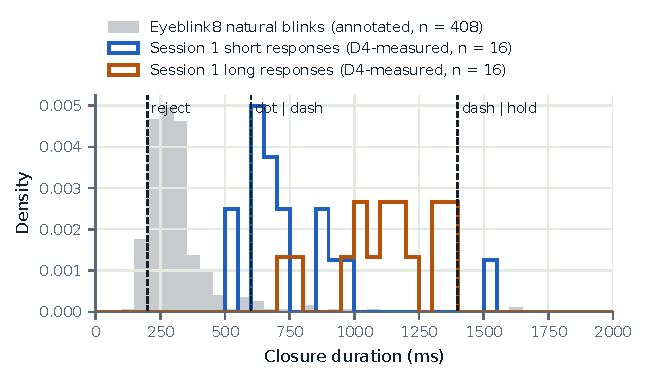
\includegraphics[width=0.66\textwidth]{C2_durations}
  \Description{Histogram of closure durations from 0 to 2000 ms. Eyeblink8 natural blinks cluster around 200 to 350 ms. Session 1 short responses, measured by D4, cluster around 600 to 900 ms, mostly to the right of the 600 ms dot-dash line. Long responses spread from about 700 to 1400 ms.}
  \caption{Closure durations against the default segmenter bands: annotated natural blinks of other people
  (Eyeblink8) and the author's short and long responses in session 1, as measured by D4 (not labelled).}
  \label{fig:durations}
\end{figure*}

\paragraph{Winks closed both eyes.} The wink detector (D5) found none of the author's winks. In every one of the
\CS{sWinks} wink responses, the other eye's blendshape score was at or above 0.3 when the winking eye was most
closed (median \CS{sWinkOtherPeak}, against \CS{sWinkPeak} for the winking eye). D5 requires it to stay below 0.3.
Either the author's winks partly closed the other eye, or the blendshape scores of the two eyes move together. One
session cannot tell these apart, but a fixed limit on the other eye did not work here.

\begin{table}[t]
  \caption{Session 1 by detector: false triggers per minute while reading (without $\to$ with the reject
  window); cue responses whose longest detected closure fell in the cued band; and median measured duration of
  short and long responses.}
  \label{tab:session}
  \small
  \resizebox{\columnwidth}{!}{\begin{tabular}{llllrr}
\toprule
ID & Detector & Reading FT/min & Correct band & Short (ms) & Long (ms) \\
\midrule
D1 & EAR, fixed 0.21 & 12.7 $\to$ 2.7 & 13/33 & 702 & 1242 \\
D2 & EAR, calibrated & 10.7 $\to$ 1.0 & 15/33 & 635 & 1153 \\
D3 & Blendshape, fixed 0.5 & 10.0 $\to$ 0.3 & 18/33 & 664 & 1118 \\
D4 & Blendshape, calibrated & 11.7 $\to$ 2.0 & 17/33 & 684 & 1126 \\
D5 & Wink (blendshape, calibrated) & 0.3 $\to$ 0.3 & 0/31 & -- & -- \\
\bottomrule
\end{tabular}
}
\end{table}

%% ---------------------------------------------------------------------------------------------
\section{Discussion}

A duration reject window is an attractive defence against spontaneous blinks because it needs no model of the
user. The public videos show that its effect depends on the signal it is applied to. The blendshape detector
measured natural blinks as short enough that most fell inside a \CS{rejectMs}\,ms window. The fixed EAR threshold
measured the same blinks as longer, so the same window removed few. A reject window therefore has to be chosen for
the signal and threshold in use, not carried over from published blink durations alone.

The single session points to the other half of the problem: deliberate closures have to be reliably longer than the
window, and the dot--dash boundary has to fit the person. The author's cued short closures, measured from the
camera, mostly exceeded the default dot limit. With the defaults, most dots would have been typed as dashes. A
per-user timing calibration, analogous to the threshold calibration, is the natural next step, and the planned
study would have tested one.

Frame rate matters for both. At 10\,fps a frame lasts 100\,ms, half the reject window, so durations near the
window's edge cannot be measured reliably. The camera in this session dropped to about 10\,fps for long stretches, apparently through its automatic
exposure; a deployed system would need to detect and report this.

\section{Limitations}

The preregistered study was not completed; none of its confirmatory hypotheses was tested on the author's data,
and the typing study was not run. The public-video analysis is not blind and covers four people in eight videos.
The session results come from one session of one person, who also designed the system, knew the hypotheses and
checked the response types.
Session durations are measured by detectors, not labelled, and the response types were checked against
placeholder windows, not exact closure times. The camera ran below the planned frame rate. No one with a motor
impairment used the system, and no clinical claim is made.

\section{Ethics and Data}

No ethics review was sought. The only participant is the author, and the public videos are used under their
published licence (GPL-3.0). The app processes video on the device and logs only per-frame features; no faces,
video or names are published. The session's features may be released with a datasheet
(\texttt{data/DATASHEET.md}).

\section{Use of AI Tools}

The software, the analysis code, the preregistration text and every section of this paper were drafted by an AI
coding agent (Claude Code, model Claude Opus 5.5, Anthropic), from a project plan written by the author. The
author recorded and checked the session, made the study decisions recorded in the preregistration's Deviations,
and reviews and edits the text. No number in this paper was written by hand: all come from the analysis scripts
run on the logged data and the public dataset. \texttt{AI\_USE.md} in the repository gives the full record.
% [HUMAN] Review this statement against AI_USE.md and edit it in your own words.

\section{Conclusion}

MorsEye shows that blink-based Morse typing can run entirely in a browser on a laptop webcam, but also how much
depends on timing. On other people's natural blinks, a \CS{rejectMs}\,ms reject window more than halved false
triggers with a blendshape detector but barely changed them with a fixed EAR threshold. In one exploratory session,
the default dot limit was too short for the author's deliberate closures. Choosing the reject window and the
dot--dash boundary per signal and per person, and testing that choice in the study this project planned, is the
work that remains.

\bibliographystyle{ACM-Reference-Format}
\bibliography{references}

\end{document}
